\pdfoutput=1
\documentclass[pra,twocolumn,showpacs,amsmath,amssymb]{revtex4-2}

\usepackage{graphicx}%Include figure files
\usepackage{dcolumn}%Align table columns on decimal point
\usepackage{bm}% bold math
\usepackage[section]{placeins} %force no floats before section
\usepackage{float}

\setlength{\parskip}{1em}

%\nofiles

\begin{document}

\title{Project 2: Deterministic Chaos in Classical 1D Scattering}


\author{Christopher McGlinn}
\affiliation{Department of Physics and Astronomy, University
of Delaware, Newark, DE 19716-2570, USA}

\begin{abstract}
We explore the motion of two point masses in one dimension. The two masses move in the vertical axis and experience gravity. As the masses move, they experience elastic collision when they are at the same location. The lower mass also "bounces" off of a floor, thus reversing direction with equal velocity. Given initial conditions, it is shown that chaos can occur with the system. We will also show that different masses can result in more or less chaotic systems. To show this we explore a Poincare cross-section of the system as well as show basic plots of the positions of each mass.
\end{abstract}

\pacs{13.85.Dz}


\maketitle

\section{Introduction} \label{sec:intro}

It is important to understand how and when chaos can occur within a system. Since initially pioneered by people such as Henry Poincare in the 1880s, chaos theory has since become an important field of study in mathematics. Chaos, in this interpretation, describes a system in which minuscule changes in initial conditions cause drastic changes in results. While the systems seem to represent random outcomes, the reality is that they can be accurately predicted through analysis. 
\par Our system explores the apparent chaotic nature of two masses. In this system, the two point masses scatter off of each other and a floor through elastic collision. This ensures that the energy of the system is preserved throughout its lifespan. We also restrict the system to one vertical dimension. The only force acting on this system is the gravitational force. The floor of this system is location at \(x = 0\). We are given initial mass, position, and velocity conditions \(m_1, m_2, x_{1_0}, x_{2_0}, v_{1_0}, v_{2_0}\). The equation that governs a single particle is as such, 
\begin{eqnarray}
X(t) = -\frac{g}{2}t^2 + v_0 t + x_0
\end{eqnarray}
\par When the particle hits the floor, the collision is elastic so the magnitude of velocity before the collision is equal to the magnitude after the collision. However, the direction after the collision is opposite of the direction before.
\par When we introduce a second mass into the system, this causes collisions between the masses. In this system the collisions are elastic, and thus both the energy and the momentum of the system is conserved. This garners the following equation:
\begin{eqnarray}
m_1 v_{1_b} + m_2 v_{2_b} = m_1 v_{1_a} + m_2 v_{2_a}
\end{eqnarray}
where b stands for before and a stands for after.
\par With this relationship, we will evaluate the system and show its chaotic nature.

\section{Method} \label{sec:method}

First we must define the set of variables for the system. To begin we will introduce a set of dimensionless variables to govern the interactions in the system. We will start off by defining a variable \(m = m_1 + m_2\) and the following sets of equations:
\begin{align}
\bar{x} &= \frac{x}{x_o} & d\bar{x} &= \frac{dx}{x_o} \notag \\
\bar{v} &= \frac{v}{v_o} & d\bar{v} &= \frac{dv}{v_o} \notag \\
\bar{t} &= \frac{t}{t_o} & d\bar{t} &= \frac{dt}{t_o} \notag \\
\bar{E} &= \frac{E}{E} \notag
\end{align}
This gives us the following equation:
\begin{align}
    \bar{E} = \frac{1}{2} \frac{m_1}{E} v_{o_1}^2 \bar{v_1}^2 + \frac{1}{2} \frac{m_2}{E} v_{o_2}^2\bar{v_2}^2 + \frac{m_1}{E} x_{o_1} x_1 + \frac{m_2}{E} x_{o_2} x_2 \notag
\end{align}
We can then define the normalization variables as such:
\begin{align}
v_o &= \sqrt{\frac{m}{E}} & t_o &= \sqrt{\frac{m}{E}} & x_o &= \frac{mg}{E} \notag
\end{align}
This gives us a new, normalized equation for the energy:
\begin{align}
\bar{E} = 1 = \frac{1}{2} \frac{m_1}{m} \bar{v_1}^2 + \frac{1}{2} \frac{m_2}{m} \bar{v_2}^2 + \frac{m_1}{m} x_1 + \frac{m_2}{m} x_2
\end{align}
Furthermore, we can define a recursive relationship between two associated times for each of the values as such:
\begin{align}
v_{1_i+1} &= v_{1_i} - g \Delta t\\
x_{1_i+1} &= x_{1_i} + \frac{v_{1_i+1} + v_{1_i}}{2} \Delta t\\
v_{2_i+1} &= v_{2_i} - g \Delta t\\
x_{2_i+1} &= x_{2_i} + \frac{v_{2_i+1} + v_{2_i}}{2} \Delta t
\end{align}
This uses the midpoint method where the collisions are calculated as "midpoints" between two different times. The midpoint method is capable of accurately portraying the system given its constant acceleration. This method does incur a certain amount of error to it, but, given a sufficiently small \(\Delta t\), it is negligible.
\par To explore the chaos of the system appropriately, we will review three different scenarios: \(\frac{m_2}{m_1} = 0.5\), \(\frac{m_2}{m_1} = 1\), \(\frac{m_2}{m_1} = 9\). In each of these scenarios we will use the following initial conditions: \(m_1 =\) 1 kg, \(x_1 =\) 1 m, \(v_1 =\) 0 m/s, \(x_2 =\) 3 m, and \(v_2 =\) 0 m/s. Given these three scenarios we will construct a Poincare cross-section of \(v_2\) vs \(x_2\) at times when the masses collide.
Also, to explore the chaotic nature of the system we will introduce the autocorrelation function:
\begin{eqnarray}
C(\tau) = \int_{0}^{\infty} [x(t) - \bar{x}][x(t + \tau) - \bar{x}]dt
\end{eqnarray}
where \(\bar{x}\), in this equation, is the average value of the system. This function will be constant or oscillating for normal systems and will decay to zero for chaotic systems. Thus we will be able to test which of our given scenarios is in fact chaotic.
\par This function can be expressed in more discreet terms with the function: 
\begin{eqnarray}
A(r) = \frac{1}{N-r} \sum_{i=1}^{N-r} [x(i) - \bar{x}][x(i + r) - \bar{x}]
\end{eqnarray}
With this function we will input the values from the recursive formulas and be able to visibly see the chaotic nature of this system.

\begin{figure}[t!]
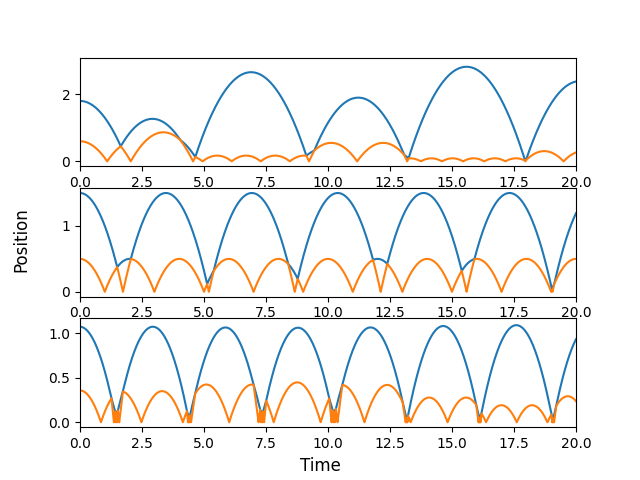
\includegraphics[scale=0.50]{x.png}
\caption{Position of masses $m_2$ and $m_1$ with respect to time for \(\frac{m_2}{m_1} = 0.5\), \(\frac{m_2}{m_1} = 1\), and \(\frac{m_2}{m_1} = 9\) respectively.}\label{position}
\end{figure}

\section{Results} \label{sec:results}

First we will explore the behavior of the system over time. As we see in Fig 1, the movement of masses 1 and 2 change quite drastically depending on their relative mass. As we see with the cases \(\frac{m_2}{m_1} = 0.5\), slight changes in the mass causes a drastic change in the "predictability" of the system. There also appears to be a bit of chaos in the situation of \(\frac{m_2}{m_1} = 9\) where the peak varies as time increases, unlike with \(\frac{m_2}{m_1} = 1\). Comparing all of the systems shows that an increase in mass also increases the frequency of collisions in the system.
\par In order to get a glimpse into the chaotic nature of the system we will look at the Poincare cross-section of each scenario. This cross section displays the points in which a collision occurs.

\begin{figure}[t!]
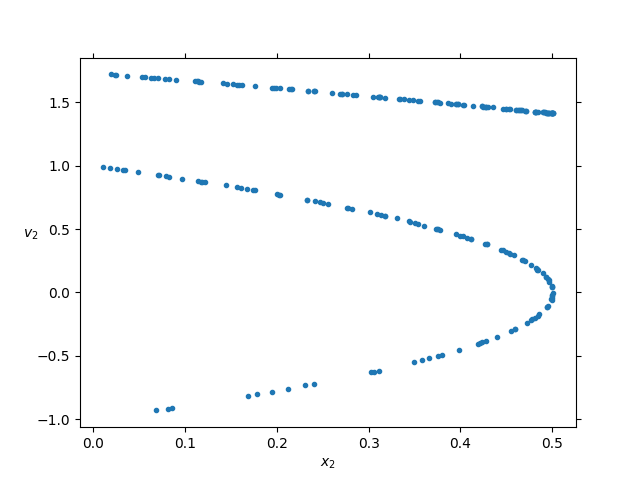
\includegraphics[scale=0.50]{Poincare1.png}
\caption{Poincare cross-section for \(\frac{m_2}{m_1} = 1\)}\label{Poincare1}
\end{figure}

\begin{figure}[t!]
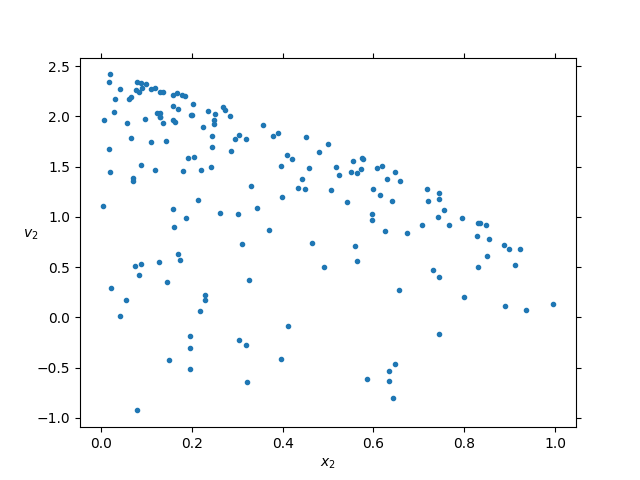
\includegraphics[scale=0.50]{Poincare0.5.png}
\caption{Poincare cross-section for \(\frac{m_2}{m_1} = 0.5\)}\label{Poincare0.5}
\end{figure}

\begin{figure}[t!]
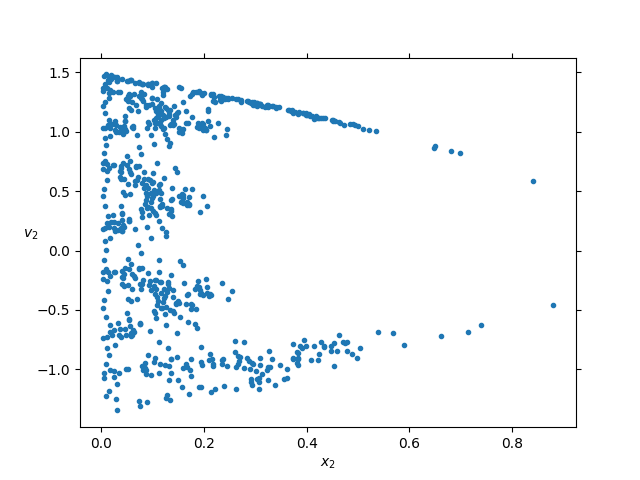
\includegraphics[scale=0.50]{Poincare9.png}
\caption{Poincare cross-section for \(\frac{m_2}{m_1} = 9\).}\label{Poincare9}
\end{figure}

In figure 2 we see that there is predictability in the system. There are areas in which a collision does not occur and the system follows a parabolic path. This has a peak at which the velocities of both masses are zero and the  
\par However, looking at figures 3 and 4, we notice that the system easily evolves into chaos. Figure 3 displays a system of unpredictability, with collisions occurring seemingly everywhere within the parabolic limit. It is quite apparent that the system is chaotic.
\par Finally with figure 4 we see some signs of predictability in the system with a portion of the empty space we saw from figure 2. However, the small parabolic pockets lend to the somewhat subtle chaotic nature of this scenario.
\par Finally we can look at the autocorrelation function over time to further analyse the system at in each scenario. The autocorrelation function will give us a better insight into how chaotic each system is.

\begin{figure}[t!]
\includegraphics[scale=0.50]{corr.png}
\caption{Autocorrelation function of mass 2 for \(\frac{m_2}{m_1} = 0.5\), \(\frac{m_2}{m_1} = 1\), and \(\frac{m_2}{m_1} = 9\) respectively.}\label{autocorr}
\end{figure}

As we see here, each of the three scenarios are somewhat chaotic. In scenarios \(\frac{m_2}{m_1} = 1\) and \(\frac{m_2}{m_1} = 9\), the amplitudes of the peaks decay over time. However, the amplitude for \(\frac{m_2}{m_1} = 9\) decays more rapidly than with \(\frac{m_2}{m_1} = 1\). Finally, as we could predict with \(\frac{m_2}{m_1} = 0.5\), the system rapidly decays to 0 and hovers around the point, thus validating the chaotic nature of the system.
\p It is easier to see the chaotic nature of the case of $ \frac{m_2}{m_1} = 9 $ if you analyze it a bit more closely. First by looking at the poincare for different scenarios.

\begin{figure}[t!]
\includegraphics[scale=0.50]{poincare.png}
\caption{Poincare of mass 2 for \(\frac{m_2}{m_1} = 9\) at different initial values of $x_2$}\label{poin9}
\end{figure}

As shown in Fig. 6, while there are minor changes to the initial conditions, the system shows a drastic change in the number of collisions. This chaos can be see by looking at the autocorrelation over a longer time period.

\begin{figure}[t!]
\includegraphics[scale=0.50]{corr3.png}
\caption{Autocorrelation function of mass 2 for \(\frac{m_2}{m_1} = 9\)}\label{autocorr9}
\end{figure}

\par As you can see in Fig. 7, while the amplitude of the autocorrelation decreases to zero over time, the amplitude also experiences a sinusoidal variation.

\section{Conclusion} \label{sec:conclusion}

After analyzing the systems we were able to validate the apparently aperiodic nature of this system. Looking at a system such as this, we can validate the very nature of chaotic systems and how they evolve over time. However, despite their apparent unpredictable natures, we are able to see some predictability in the way they evolve and our ability to analyse the systems.

\begin{thebibliography}{9}
\bibitem{}Nicholas J. Giordano and Hisao Nakanish, \emph{Computational Physics}, (Pearson Prentice Hall, Upper Saddle River NJ,2006).
\bibitem{}N. D. Whelan, D. A. Goodings, and J. K. Cannizzo, “Two balls in one dimension with gravity,” \emph{Physical Review A}, Vol. 42, No. 2, p. 742, 1990.
\end{thebibliography}

\end{document}